\documentclass[11pt]{article}

% Change "review" to "final" to generate the final (sometimes called camera-ready) version.
% Change to "preprint" to generate a non-anonymous version with page numbers.
\usepackage[review]{acl}

% Standard package includes
\usepackage{times}
\usepackage{latexsym}

% For proper rendering and hyphenation of words containing Latin characters (including in bib files)
\usepackage[T1]{fontenc}
% This assumes your files are encoded as UTF8
\usepackage[utf8]{inputenc}

% This is not strictly necessary, and may be commented out,
% but it will improve the layout of the manuscript,
% and will typically save some space.
\usepackage{microtype}

% This is also not strictly necessary, and may be commented out.
% However, it will improve the aesthetics of text in
% the typewriter font.
\usepackage{inconsolata}

% Including images in your LaTeX document requires adding
% additional package(s)
\usepackage{graphicx}
\usepackage{booktabs}
\usepackage{amsmath}
\usepackage{enumitem}
\usepackage{float}
\usepackage{caption}
\usepackage{subcaption}
\usepackage{listings}
\usepackage{xcolor}
\usepackage{titlesec}

\lstset{
  basicstyle=\ttfamily\footnotesize,
  breaklines=true,
  columns=fullflexible,
  frame=single,
  backgroundcolor=\color{black!3},
  breakindent=0pt,
  xleftmargin=2pt,
  xrightmargin=2pt,
}

\title{BranchMem: Boundary Conditions for Asynchronous Semantic Agent Memory Merging}

\author{Anonymous submission}

% Modest, standard space-saving: tighter table rows and less padding
% around floats. Does not change font size or content, only whitespace.
\renewcommand{\arraystretch}{0.92}
\setlength{\textfloatsep}{6pt plus 1pt minus 2pt}
\setlength{\intextsep}{6pt plus 1pt minus 2pt}
\setlength{\abovecaptionskip}{3pt}
\setlength{\belowcaptionskip}{2pt}

% Tighter spacing around section/subsection/paragraph headings (titlesec
% only changes spacing here, not ACL's required font/size/weight for
% these headings, via \titlespacing* rather than \titleformat).
\titlespacing*{\section}{0pt}{6pt plus 1pt minus 1pt}{3pt plus 1pt minus 1pt}
\titlespacing*{\subsection}{0pt}{5pt plus 1pt minus 1pt}{2pt plus 1pt minus 1pt}
\titlespacing*{\paragraph}{0pt}{4pt plus 1pt minus 1pt}{0.5em}
\setlength{\parskip}{0pt}

\begin{document}
\maketitle

\begin{abstract}
Reconciling two branches of an LLM agent's memory that diverged while
disconnected differs from live multi-agent coordination and
single-timeline freshness: no shared clock, no live negotiation. We
introduce \textsc{BranchMem}, a preregistered benchmark and harness to
identify \emph{when} such merging is reliable, not to claim it solved.
Ancestor-aware LLM merging beats naive baselines by wide margins, but only
when provenance carries a legible reliability signal: strip it and the LLM
collapses to naive-baseline territory, while \textsc{ConfidenceRuleMerge}
--- a deterministic rule reading the same field --- matches or beats it,
the strongest baseline here. On real, branch-forked MemoryAgentBench
content, where no such field exists, the ranking inverts: across $230$
conflicts the LLM never guesses, correctly flagging the absent signal,
which accuracy alone penalizes as error. We report abstention-aware
metrics showing calibrated abstention is correct once a signal is absent.
Cheap conflict detection is a separate, mixed result on a harder, balanced
test set. We release the harness, preregistered plan, and every cached
call.
\end{abstract}

\section{Introduction}
\label{sec:intro}

Language-model agents increasingly carry a persistent, natural-language
\emph{belief state} that is naturally replicated across devices, sessions,
or replicas. When two replicas operate while disconnected --- a phone
assistant used offline while a desktop copy keeps learning --- each
accumulates its own updates; on reconnection, the two \emph{branches} of
memory must be merged into one.

This paper is about \emph{when}, not whether, that merge can be trusted:
our central finding is a boundary condition, not a method. LLM-mediated
merging is reliable exactly when branch provenance carries a legible
reliability signal, a deterministic rule reads it just as well, and, on
real content where no such signal is engineered in, the right behavior is
to abstain rather than guess, which accuracy alone scores as a mistake.

The asynchronous partition-and-merge problem differs from three related
lines of work. It is not \emph{live multi-agent coordination}: systems such
as S-Bus \citep{khan2026sbus} abort or retry conflicting commits via
optimistic concurrency control, presupposing agents share a substrate
online --- our branches were never online together, so there is nothing to
abort, only two already-committed histories to reconcile. Nor is it
\emph{single-timeline temporal freshness}: on one ordered timeline a
deterministic \texttt{max(serial)} rule beats asking the LLM to judge
freshness \citep{reddy2026freshness}, but disconnected branches share
\emph{no clock}; ``later'' on one branch's timestamp says nothing about
correctness relative to the other. Nor is it \emph{structured, CRDT-style
replication}: CRDTs \citep{shapiro2011crdt} and convergent-log substrates
\citep{sarkar2026grite} resolve divergence with a commutative merge
function so any two replicas provably reconcile; free-form language has no
such operator --- whether ``the user prefers window seats'' and ``prefers
aisle seats'' should merge, split, or flag is a semantic judgement,
precisely where an LLM might help over naive alternatives
(last-writer-wins, keep everything, drop a branch), if it buys anything
over these cheap defaults at all.

\paragraph{Why abstention matters here.} A wrong merge silently corrupts
the agent's belief, and every downstream decision inherits the error; we
cannot abort, as coordination systems can, since branches already
committed offline. When no signal distinguishes the correct value, forcing
a commit is a coin flip dressed as an answer; flagging it trades a lower
accuracy score for a lower chance of propagating a wrong belief --- a
tradeoff accuracy alone hides (Section~\ref{sec:abstention}).

We formalize this problem and build \textsc{BranchMem}, a harness that
forks a common-ancestor memory, applies independent scripted updates to two
branches, and scores how well merge strategies recover a construction-time
ground truth, studying three questions: \textbf{RQ1}, does an explicit
\emph{three-way} LLM merge---ancestor plus both branches---beat naive
last-writer-wins and concatenation? \textbf{RQ2}, can conflict
\emph{detection} be done cheaply (embedding similarity, a small NLI model)
instead of with an LLM judge? \textbf{RQ3}, does reconciled memory beat
discarding one branch entirely (the post-hoc analogue of an abort)?

Hypotheses, statistical tests, effect sizes, and falsification criteria
were locked \emph{before} the confirmatory run; every subsequent addition
is disclosed as post-hoc and kept separate
(\texttt{ANALYSIS\_PLAN\_ADDENDUM.md}), including results unfavorable to the
headline claim (Sections~\ref{sec:ablations}, \ref{sec:mab-negative}). Our
contributions: (i) we formalize asynchronous partition-and-merge for semantic agent
memory, distinct from live coordination, single-timeline freshness, and
CRDT-style replication; (ii) we introduce \textsc{BranchMem}, a
reproducible benchmark and harness for forked semantic memories, every
real model call cached and released; (iii) we show LLM-mediated merging
beats naive baselines only when provenance carries a legible reliability
signal (RQ1, RQ3); (iv) we show a deterministic, confidence-based rule
(\textsc{ConfidenceRuleMerge}) is a strong baseline that matches or beats
the LLM under the current construction (Section~\ref{sec:ablations});
(v) we add abstention-aware evaluation (Section~\ref{sec:abstention}) ---
commit rate, conditional accuracy, and expected utility --- showing when
\textsc{flagged\_unresolved} is safer than forcing a resolution;
(vi) we evaluate conflict detectors on a balanced conflict/non-conflict set
(Section~\ref{sec:detectors-balanced}), not only positive examples, giving
RQ2 real precision, not just recall; and (vii) we report a real-content
MemoryAgentBench extension (Section~\ref{sec:mab-negative}) showing the
synthetic provenance signal does not automatically exist in realistic
memory data --- the boundary condition this paper is built around.

\section{Related Work}
\label{sec:related-work}

Four further points of comparison --- agent memory benchmarks
\citep{shinn2023reflexion,packer2023memgpt,hu2025memoryagentbench}, live
multi-agent coordination (S-Bus's \emph{prevention/abort} model,
\citealp{khan2026sbus}), single-timeline temporal freshness (a
deterministic ``pick the maximum serial'' recipe,
\citealp{reddy2026freshness}), and conflict detection via embeddings/NLI
\citep{longpre2021knowledge,lewis2020rag,reimers2019sentencebert} --- are
each close enough to our setting to warrant full discussion; we give it in
Appendix~\ref{sec:related-work-extended} rather than here, since the core
distinctions are already established in Section~\ref{sec:intro}, and the
detector background supports only RQ2, not the paper's central claim.

\subsection{Structured replication, CRDTs, and local-first software}
CRDTs \citep{shapiro2011crdt} and operational transformation
\citep{ellis1989concurrency} give provably convergent, commutative merge
for structured data; convergent-log agent substrates \citep{sarkar2026grite}
and local-first software \citep{kleppmann2019localfirst} build on the same
primitives. Convergence needs a merge operator with lattice-like structure,
which free-form language lacks; \textsc{BranchMem} studies what to do
without one, using an LLM as a best-effort reconciler rather than a
guaranteed-convergent one.

\subsection{Abstention and selective prediction}
Selective classification \citep{elyaniv2010selective,geifman2017selective}
formalizes the coverage-risk tradeoff used in Section~\ref{sec:abstention}:
a classifier that may abstain trades coverage against risk rather than
being forced to one accuracy number. \textsc{flagged\_unresolved} is a
selective-prediction abstention; accuracy alone cannot distinguish a
calibrated abstention from a wrong guess.

\section{Problem Formulation and Method}

\subsection{Branch, fork, and merge}
\label{sec:formulation}

We represent memory as a set of \emph{facts}, each a canonicalized tuple
$(\textit{entity}, \textit{predicate}, \textit{value})$ with metadata
$(\textit{source}, \textit{confidence}, \textit{timestamp})$, where
$\textit{source}\in\{\texttt{user}, \texttt{observation}, \texttt{inference}\}$.
The pair $k=(\textit{entity},\textit{predicate})$ is a \emph{key}; the current
value at a key is the fact with the latest branch-local timestamp for that key.

A \emph{common ancestor} $M_0$ is forked into branches $A$ and $B$, each
initialized as a copy of $M_0$. Each branch then applies an independent
stream of scripted updates, superseding prior facts at a key while retaining
full history. Every key touched by both branches yields a \emph{conflict
pair}. A merge strategy consumes $(M_0, A, B)$ and returns a reconciled fact
set in which each key resolves to \textsc{kept} (one branch's value, or
agreement), \textsc{merged} (a reconciled value), \textsc{dropped} (lost), or
\textsc{flagged\_unresolved} (deferred to the user). Ground-truth conflict
labels and correct values are attached \emph{by construction} at
scenario-generation time, never inferred afterward.

\subsection{Merge strategies}

We compare four families, five strategies in total.

\noindent\textbf{LastWriterWins (LWW).} At each conflicting key, keep the fact
with the later timestamp --- the strategy the freshness recipe
\citep{reddy2026freshness} would reduce to, but uninformative here since the
branches have no shared clock.

\noindent\textbf{NaiveConcat.} Keep every current fact from both branches:
never drops information, but never resolves a genuine contradiction either ---
both conflicting values survive, so downstream reads see an inconsistent store.

\noindent\textbf{BranchDiscard.} On \emph{any} detected key collision, discard
one branch's entire post-fork update set (including non-conflicting additions)
and keep the other --- the post-hoc analogue of an abort. Two policies:
\texttt{always\_b} (always drop $B$) and \texttt{fewer\_updates} (drop the
branch with fewer updates); facts identical to the kept branch's value are not
counted as lost.

\noindent\textbf{ThreeWayLLMMerge (proposed).} Analogous to a three-way file
merge, the LLM gets the common ancestor's value for each conflicting key plus
both branches' current value, source, and confidence, and reconciles each
with a one-sentence justification or flags it unresolvable. Non-conflicting
keys resolve deterministically in code; only genuine collisions reach the
model, batched into one call per merge. The system prompt instructs it to use
source/confidence and ancestor context---\emph{not} timestamps, since
disconnected branches share no clock---and to flag rather than guess absent a
distinguishing signal (full prompt in Appendix~\ref{sec:prompt}; worked
example in Appendix~\ref{sec:example}).

\subsection{Conflict detectors (RQ2)}

Merge strategies identify candidate conflicts structurally (same key,
differing current value), which is realistic for a canonicalized fact store.
RQ2 asks a separate question: can we \emph{detect} whether two
natural-language values genuinely conflict without an LLM? We compare three
detectors, treating the LLM judge as the reference standard, not a competitor.

\noindent\textbf{EmbeddingConflictDetector.} Since candidate pairs already
share a key, low cosine similarity between the two \emph{value} strings
(sentence embeddings, \texttt{all-MiniLM-L6-v2}, \citealp{reimers2019sentencebert})
signals a real conflict, high similarity a paraphrase; a calibrated
threshold decides.

\noindent\textbf{NLIConflictDetector.} A small NLI cross-encoder
(\texttt{nli-deberta-v3-small}) scores the contradiction probability between
the two facts phrased as short sentences; a calibrated threshold decides.

\noindent\textbf{LLMJudgeConflictDetector.} An LLM judges whether the two
values conflict --- the RQ2 reference standard. Both cheap detectors run
locally at no API cost; the LLM judge does not.

\subsection{Scenario generator and conflict taxonomy}
\label{sec:gen}

The generator builds fully deterministic scenarios (given a seed) from a fixed
pool of entities, \emph{objective} predicates (with a fact-of-the-matter), and
\emph{subjective} predicates (without one). Each scenario forks a
$4$-fact ancestor and scripts three kinds of divergence:

\noindent\textbf{Orthogonal.} A key touched by exactly one branch (a new,
non-contradictory addition). The correct behavior is to \emph{preserve} it;
this is where \textsc{BranchDiscard} structurally loses information.

\noindent\textbf{Resolvable conflict.} Both branches update the same key with
contradicting values, and there \emph{is} a single correct reconciled value,
tied to a \emph{source-reliability signal}: one branch's update is
\texttt{user}-sourced with high confidence, the other
\texttt{inference}-sourced with low confidence, and ground truth is the
user-sourced value---with $15\%$ noise, so a strategy cannot get a free
$100\%$ by blindly trusting the user source. This signal was not incidental;
it resolves a construct-validity problem uncovered in piloting
(Section~\ref{sec:discussion}).

\noindent\textbf{Ambiguous conflict.} Both branches update the same
\emph{subjective} key with different values and the \emph{same}
source/confidence---there is deliberately no distinguishing signal, so the only
correct behavior is to \textsc{flag}, not guess. Ground truth is ``unresolved.''

A separate parameter, \texttt{timestamp\_correlates\_with\_correctness}, set to
$0.5$, controls only whether the correct branch also happens to carry the later
timestamp---uninformative about correctness at $0.5$, the realistic
asynchronous case, so LWW is neither trivially right nor trivially wrong. This
value and the source-reliability construction were preregistered before the
locked run. Downstream questions are generated one per conflict pair and per
orthogonal addition, scored against the generator's ground truth by Python
equality, never against any model's opinion.

\subsection{MemoryAgentBench extension}
\label{sec:mab}

To test realistic content, we extend MemoryAgentBench's Fact Consolidation task
\citep{hu2025memoryagentbench} with a branch-fork step. Since its published
data exposes only a flattened context string, we built a 38-template regex
parser recovering $(entity, predicate, value)$ triples at $99.9\%$ coverage
over $18{,}337$ context lines. Coverage alone does not establish correctness,
so we additionally ran an \emph{author self-audit} (not
independent validation, explicitly labeled as such) on $50$ of the
$51{,}314$ parsed triples: $0$ errors ($95\%$ Clopper--Pearson CI
$[0,0.071]$). End-to-end validation against the live dataset surfaced two
construction bugs (Section~\ref{sec:discussion}); after fixing them, LWW
accuracy clustered near chance ($49$--$56\%$) across $17{,}816$ conflict
pairs, as expected for an unbiased construction. Fact Consolidation is
deterministic, so this extension yields only resolvable and orthogonal
divergences; our \emph{primary} experiment runs on the synthetic generator
instead, where the resolvable/ambiguous mix is controllable, and the MAB
extension is a validated secondary path (Section~\ref{sec:mab-negative}), not
part of the locked analysis.

One difference matters for Section~\ref{sec:mab-negative}: the MAB extension
does \emph{not} construct a source-reliability signal --- its
\texttt{UpdateSpec}s inherit the dataset's own provenance, so both branches
default to \texttt{source="observation"}, \texttt{confidence=1.0}, no
\texttt{user}-vs.-\texttt{inference} distinction. This is not an oversight to
patch; real, reconstructed content lacks the clean annotation we
hand-designed for the synthetic generator (Section~\ref{sec:gen}), and we
treat that absence as the realistic case worth measuring.

\section{Experimental Setup}
\label{sec:setup}

\paragraph{Preregistration.} After a pilot phase used to fix bugs and calibrate
thresholds, we committed an analysis plan specifying the hypotheses, statistical
tests, minimum effect sizes, F1 tolerance, detector thresholds, sample size, and
falsification criteria \emph{before} the locked run. The locked run then executed
exactly that plan with no parameter changes.

\paragraph{Model.} All LLM-dependent components (\textsc{ThreeWayLLMMerge},
\textsc{LLMJudge}) use \texttt{gpt-5.4-nano}, the cheapest OpenAI model
available to us. This was an explicit cost-minimization constraint, not a
capability claim; whether effects hold with stronger models is future work.

\paragraph{Scenarios and seeds.} The locked run uses $n{=}60$ scenarios ($20$
each at divergence spans $4.0$, $10.0$, $20.0$), seed $2026$, yielding $180$
ground-truth conflict pairs ($120$ resolvable, $60$ ambiguous). Each scenario
has $1$ entity, a $4$-fact ancestor, two orthogonal additions per branch
(Appendix~\ref{sec:config} notes a documentation correction here), two
resolvable conflicts, and one ambiguous conflict.

\paragraph{Detector calibration.} Embedding and NLI thresholds were swept
against the $60$ ground-truth conflict pairs of the \emph{pilot} set (held out
from the locked set); precision was $1.0$ across the entire sweep for both
detectors---only false negatives. We locked embedding threshold $0.80$
(start of its F1 plateau) and NLI threshold $0.20$ (middle of its
higher-F1 plateau), choosing plateau interiors for robustness to
distribution shift (full sweep in Appendix~\ref{sec:calibration}).

\paragraph{Statistics.} For RQ1/RQ3 we use per-scenario paired accuracy
differences, a paired Wilcoxon signed-rank test per comparison (chosen over
a $t$-test since per-scenario accuracy is a bounded proportion over few
questions), Holm--Bonferroni correction across the four confirmatory
comparisons, and $2000$-resample paired bootstrap $95\%$ CIs. The minimum
meaningful effect is $0.10$ accuracy (preregistered from pilot variance;
support requires both corrected significance and a CI lower bound above
$0.10$). For RQ2 we use a fixed $0.05$ F1 tolerance band relative to the
LLM judge---no significance test---matching the build spec's example value.

\paragraph{Non-determinism.} Pilot resampling showed a low flip rate
($1/15{=}6.7\%$ for the merge, $0/10$ for the judge), so the locked run calls
each LLM-dependent component once per scenario/pair rather than majority-voting,
a preregistered cost/variance tradeoff disclosed as a limitation.

\paragraph{Reproducibility.} Every real model call across pilot and locked run
($460$ calls total; $111{,}403$ input / $45{,}462$ output tokens) is
content-hash cached and committed as an auditable artifact; re-running costs
nothing once the cache is populated.

\paragraph{Post-hoc robustness checks (not preregistered).} We ran two
additional checks after the locked analysis was complete, disclosed as
exploratory rather than confirmatory: a model swap on a scenario subset, and
a secondary run on real MemoryAgentBench content. Both are described where
reported, Sections~\ref{sec:robustness}--\ref{sec:mab-negative}.

\section{Results}
\label{sec:results}

\begin{table*}[t]
  \centering
  \small
  \resizebox{\textwidth}{!}{%
  \begin{tabular}{llcccc}
    \toprule
    \textbf{Hyp.} & \textbf{Comparison} & \textbf{Mean acc.\ diff} & \textbf{95\% CI} & \textbf{Holm-adj.\ $p$} & \textbf{Supported?} \\
    \midrule
    H1 & three-way vs.\ last-writer-wins       & $+0.219$ & $[0.183, 0.252]$ & $1.2\times10^{-10}$ & \textbf{Yes} \\
    H1 & three-way vs.\ naive-concat           & $+0.236$ & $[0.205, 0.267]$ & $1.2\times10^{-10}$ & \textbf{Yes} \\
    H2 & three-way vs.\ branch-discard (always\_b)    & $+0.493$ & $[0.460, 0.526]$ & $3.7\times10^{-11}$ & \textbf{Yes} \\
    H2 & three-way vs.\ branch-discard (fewer\_updates) & $+0.493$ & $[0.460, 0.526]$ & $3.7\times10^{-11}$ & \textbf{Yes} \\
    \bottomrule
  \end{tabular}%
  }
  \caption{Confirmatory RQ1/RQ3, locked set ($n{=}60$, Holm--Bonferroni
  corrected). All four clear the preregistered $0.10$ effect ---
  \textbf{decomposed in Table~\ref{tab:category}, qualified in
  Section~\ref{sec:mab-negative}.}}
  \label{tab:confirmatory}
\end{table*}

\begin{table}[t]
  \centering
  \small
  \resizebox{\columnwidth}{!}{%
  \begin{tabular}{lccc}
    \toprule
    \textbf{Strategy} & \textbf{Orthog.} & \textbf{Resolv.} & \textbf{Ambig.} \\
    \midrule
    last\_writer\_wins            & $1.000$ & $0.508$ \tiny{$\pm.359$} & $0.000$ \\
    naive\_concat                 & $1.000$ & $0.450$ \tiny{$\pm.325$} & $0.000$ \\
    branch\_discard (always\_b)   & $0.500$ & $0.550$ \tiny{$\pm.325$} & $0.000$ \\
    branch\_discard (fewer\_upd.) & $0.500$ & $0.550$ \tiny{$\pm.325$} & $0.000$ \\
    \textsc{ConfidenceRuleMerge}$^\dagger$ (no LLM) & $1.000$ & $0.867$ & $1.000$ \\
    three\_way\_llm               & $1.000$ & $0.858$ \tiny{$\pm.275$} & $0.833$ \tiny{$\pm.373$} \\
    \bottomrule
  \end{tabular}%
  }
  \caption{Accuracy by category ($n{=}60$; SD in small type). Orthogonal
  ties; resolvable is the genuine gap, where \textsc{ConfidenceRuleMerge}
  edges out the LLM ($0.867$ vs.\ $0.858$); ambiguous is flagged by both
  confidence-aware strategies. $^\dagger$Post-hoc addition, zero LLM cost,
  not part of Table~\ref{tab:confirmatory}. Visualized in
  Figure~\ref{fig:category}.}
  \label{tab:category}
\end{table}

\begin{figure}[H]
  \centering
  \begin{subfigure}[b]{0.48\columnwidth}
    \centering
    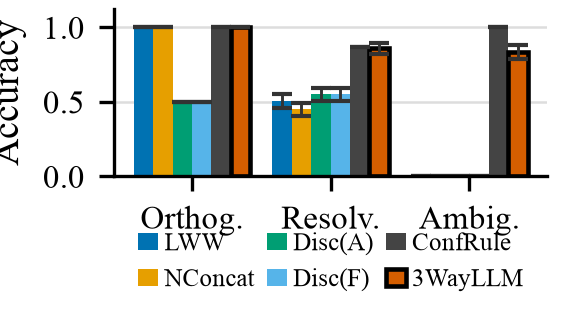
\includegraphics[width=\linewidth]{category_breakdown_a.png}
    \caption{Accuracy by category, strategy.}
    \label{fig:category-a}
  \end{subfigure}%
  \hfill
  \begin{subfigure}[b]{0.48\columnwidth}
    \centering
    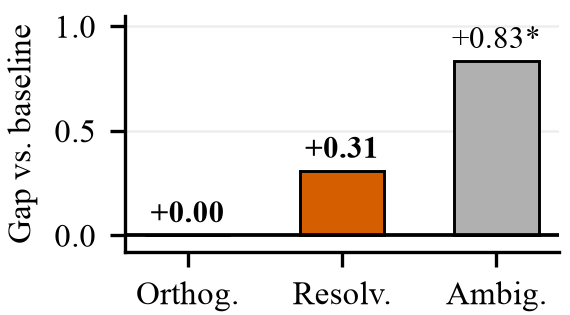
\includegraphics[width=\linewidth]{category_breakdown_b.png}
    \caption{Margin over best baseline.}
    \label{fig:category-b}
  \end{subfigure}
  \caption{Table~\ref{tab:category} visualized, with
  \textsc{ConfidenceRuleMerge} (gray, post-hoc) promoted alongside the
  locked-run strategies. (a) Black outline = \textsc{ThreeWayLLMMerge};
  \textsc{ConfidenceRuleMerge} matches or beats it on resolvable and
  ambiguous. (b) Margin over best \emph{naive} baseline: resolvable
  ($+0.31$) is genuine; ambiguous ($+0.83$, gray, $*$) is mechanically
  guaranteed.}
  \label{fig:category}
\end{figure}

\subsection{RQ1: three-way merge vs.\ naive baselines (H1) --- supported, but concentrated in one category}

Three-way merge scores $0.936$ mean downstream accuracy overall, versus $0.717$
(LWW) and $0.700$ (naive concat); both comparisons (Table~\ref{tab:confirmatory})
clear the $0.10$ minimum effect by a wide margin. Taken at face value this looks
like a broad win over naive baselines; Table~\ref{tab:category} and
Figure~\ref{fig:category} show it is concentrated, and Section~\ref{sec:ablations}
shows it is not a win over the \emph{strongest} baseline. All strategies tie at
$1.000$ on orthogonal questions, contributing nothing to the gap. On
\textbf{resolvable} conflicts, three-way merge scores $0.858$ versus
$0.45$--$0.55$ for the naive baselines: given the ancestor plus each branch's
source/confidence, the model identifies the more-reliable branch most of the
time, while the naive strategies do little better than the $\approx50\%$
chance rate implied by our timestamp-uncorrelated design. \textbf{This is the
paper's real, non-mechanical finding against naive baselines} --- though
Section~\ref{sec:ablations} shows a deterministic rule reading the same
signal scores $0.867$ here, edging out the LLM. On \textbf{ambiguous}
conflicts, three-way merge scores $0.833$ versus $0.000$ for every naive
baseline: no naive strategy can emit \textsc{flagged\_unresolved} at all, so
none could score above $0$ regardless of reasoning quality --- though again,
\textsc{ConfidenceRuleMerge} matches this by flagging exact-confidence ties
(Table~\ref{tab:category}). Section~\ref{sec:mab-negative} shows the
resolvable-conflict finding itself does not survive removing the
hand-designed reliability signal --- the single most important qualifier to
this result. Divergence duration had little effect ($0.914/0.957/0.936$ at
spans $4.0/10.0/20.0$; per-span breakdown in Appendix~\ref{sec:per-span}).
\textbf{Reframing RQ1:} \textsc{ThreeWayLLMMerge} beats naive baselines but
not the strongest provenance-aware deterministic baseline, so the LLM's
potential value must be tested where raw text or ancestor context carries
information a source/confidence field does not
(Section~\ref{sec:semantic-resolvable}).

\subsection{Ablations: the strongest baseline is deterministic abstention, not LWW}
\label{sec:ablations}

Three post-hoc ablations on the same $n{=}60$ scenarios test whether
\textsc{ThreeWayLLMMerge} needs its full source/confidence/ancestor design.
The first result reframes the whole comparison: naive last-writer-wins is
\emph{not} the strongest alternative to the LLM. \textsc{ConfidenceRuleMerge}
makes no LLM call: keep the higher-confidence branch, flag on an exact tie.
It scores $0.962$ --- \emph{higher} than
\textsc{ThreeWayLLMMerge}'s $0.936$ (paired diff $-0.026$, $95\%$ CI
$[-0.040,-0.014]$, $p{=}0.002$): a single \texttt{if}-statement outperforms the
LLM, since higher confidence is correct with probability
$1{-}$\texttt{source\_signal\_noise}${=}0.85$ by construction and ties (the
ambiguous case) are flagged just as reliably by a rule as by judgment.
\textsc{TwoWayLLMMerge} withholds the ancestor entirely; it scores $0.926$,
statistically indistinguishable from the full version ($p{=}0.29$) --- ground
truth here is tied to source/confidence, not ancestor context, so the
ancestor is not yet load-bearing in this construction.

\textbf{\textsc{RawTextLLMMerge}: withhold
\emph{everything}.} \textsc{TwoWayLLMMerge} still hands the model a structured
\texttt{confidence} field --- exactly what \textsc{ConfidenceRuleMerge} reads
directly. To isolate LLM reasoning about the raw text from reading that
field, \textsc{RawTextLLMMerge}'s prompt gives \emph{only} the entity,
predicate, and each branch's raw conflicting value --- no ancestor, source,
confidence, or timestamp. It scores $0.712$ overall --- close to the naive
baselines ($0.70$--$0.72$) and far below \textsc{ThreeWayLLMMerge} (paired
diff $+0.224$, $95\%$ CI $[0.200,0.248]$, $p{<}10^{-10}$). The category
breakdown is stark: $1.000$ orthogonal, $0.000$ \textbf{resolvable} ---
\emph{worse than every naive baseline} --- and $0.983$ ambiguous. With no
structured signal, the model does not guess from content; it flags almost
everything, exactly correct on ambiguous conflicts and exactly wrong, under
our scoring rule, on resolvable ones --- essentially none of RQ1's
resolvable-category win is attributable to the LLM reasoning about the raw
text itself.

\begin{table}[t]
  \centering
  \small
  \resizebox{\columnwidth}{!}{%
  \begin{tabular}{lc}
    \toprule
    \textbf{Strategy} & \textbf{Mean acc.} \\
    \midrule
    \textsc{ConfidenceRuleMerge} (no LLM)     & $0.962$ \\
    \textsc{ThreeWayLLMMerge} (proposed)       & $0.936$ \\
    \textsc{TwoWayLLMMerge} (no ancestor)       & $0.926$ \\
    \textsc{RawTextLLMMerge} (no metadata)      & $0.712$ \\
    \bottomrule
  \end{tabular}%
  }
  \caption{Ablations, same $n{=}60$ scenarios; exploratory, post-hoc.
  \textsc{RawTextLLMMerge} added as a later post-hoc check.}
  \label{tab:ablations}
\end{table}

\textbf{Reading.} \textsc{ConfidenceRuleMerge} also fails on real
MemoryAgentBench content (Section~\ref{sec:mab-negative}) for the same
reason --- not evidence the LLM is useless, only that this benchmark's
current construction is well-approximated by reading one metadata field.
\textsc{RawTextLLMMerge} sharpens this: without that field, the LLM's own
judgment of the raw values matches its real-content behavior, not its
synthetic resolvable-category behavior. Crediting genuine semantic reasoning
needs cases where confidence alone is insufficient \emph{and} the raw text
carries a resolvable signal, which the generator does not yet build ---
future work, not a reason to retract RQ1's aggregate result.

\subsection{RQ3: three-way merge vs.\ branch-discard (H2) --- supported by a near-mechanical margin}

Three-way merge beats both branch-discard policies by $+0.493$
(Table~\ref{tab:confirmatory}) --- the largest effect in the study, and the
one we flag as carrying the \emph{least} evidentiary weight. Both policies
scored identically ($0.443$ overall): single-entity scenarios with
symmetric update counts leave nothing for \texttt{fewer\_updates} to
distinguish, and discarding a whole branch mechanically throws away its
non-conflicting orthogonal additions, present in every scenario. Disclosed
in advance, H2 support was expected almost by construction; we report it as
\textbf{confirmation of a predicted-by-design failure mode}, not evidence
on par with Section 5.1's resolvable-conflict finding.

\subsection{RQ2: cheap detectors vs.\ LLM judge (H3) --- mixed}

Table~\ref{tab:detectors} gives the result: embedding F1 $0.957$ vs.\ judge
$0.986$ (gap $0.029$, within the $0.05$ tolerance, \textbf{supported}); NLI F1
$0.925$ (gap $0.061$, \textbf{falsified}). This is a genuine
\emph{generalization gap}, not a fixed-threshold artifact: the judge's own
F1 moved from $0.966$ on the pilot calibration set to $0.986$ on the
independently-generated, three-times-larger locked set, and bootstrapped
$95\%$ CIs on the gap itself (embedding $0.029$ $[0.006,0.056]$; NLI $0.061$
$[0.036,0.089]$) show this is consistent with ordinary sampling variation,
not a systematic drift; NLI's interval straddles $0.05$, so
\textbf{falsified} holds at the point estimate but not free of sampling
uncertainty (full detail in Appendix~\ref{sec:calibration}). Precision is
$1.0$ for every detector because every \texttt{ConflictPair} here is a
genuine conflict by construction, so $1.0$ reflects pair construction, not
measured specificity (Section~\ref{sec:detectors-balanced} adds real
negative examples). Both cheap detectors' errors are exclusively missed
conflicts, and both run $\approx\!5$--$10\times$ faster than the judge at
no API cost.

\begin{table}[t]
  \centering
  \small
  \resizebox{\columnwidth}{!}{%
  \begin{tabular}{lccc}
    \toprule
    \textbf{Detector} & \textbf{F1} & \textbf{Gap} & \textbf{$\leq 0.05$?} \\
    \midrule
    embedding ($t{=}0.80$) & $0.957$ & $0.029$ & \textbf{Yes} \\
    NLI ($t{=}0.20$)       & $0.925$ & $0.061$ & \textbf{No}  \\
    \midrule
    LLM judge (reference)  & $0.986$ & --- & --- \\
    \bottomrule
  \end{tabular}%
  }
  \caption{RQ2: conflict-detection F1 (locked set, $180$ pairs) vs.\ LLM-judge
  reference. Gap $=|$F1$_\text{cheap}-0.986|$; tolerance $0.05$.}
  \label{tab:detectors}
\end{table}

\textbf{Post-hoc: a balanced detector benchmark.}
\label{sec:detectors-balanced}
Since the locked set above has no negative examples by construction (so
precision is mechanically $1.0$), we built a balanced, hand-authored
$48$-pair set spanning six categories and re-ran all three detectors: the
embedding detector's locked-set precision turns out to be a construction
artifact (it is the \emph{weakest} on this harder set), while NLI reverses
its ``falsified'' standing (best cost-free option here). Post-hoc,
exploratory; does not change RQ2's locked result. Full setup, metrics, and
per-category breakdown in Appendix~\ref{sec:detectors-balanced-detail}.

\subsection{Does raw text ever carry the resolving signal?}
\label{sec:semantic-resolvable}

\textsc{RawTextLLMMerge} (Section~\ref{sec:ablations}) strips
source/confidence, but every ``resolvable'' conflict there still ties
ground truth \emph{only} to that metadata. We built a disjoint-seed
category, \texttt{semantic\_resolvable} ($n{=}150$, seed $3001$): identical
source/confidence on both branches, with the ancestor holding a stated
constraint at the \emph{same} key as the conflict (e.g.\ ancestor ``is
vegetarian''; branch values ``wants chicken'' vs.\ ``wants tofu''), so the
answer is recoverable only from semantic compatibility with that
constraint --- a fair test of whether raw text or ancestor semantics can
resolve a conflict on their own. Every confidence-independent strategy,
\emph{including} \textsc{ThreeWayLLMMerge} which receives the constraint,
scores \emph{exactly} $0.000$; naive baselines score $0.47$--$0.53$
(chance-level, as designed). We read this as a genuine negative result:
giving the model the necessary semantic content did not produce reliable
semantic resolution. Full construction detail, a construct-validity bug we
caught and fixed on the first run, and transcript analysis are in
Appendix~\ref{sec:semantic-resolvable-detail}.

\subsection{Post-hoc robustness checks: a more capable model, and a resolvable-category replication}
\label{sec:robustness}

Two post-hoc robustness checks --- a \texttt{gpt-5.4-mini} model swap on
the same $20$ scenarios, and a second, disjoint-seed $120$-pair
resolvable-category sample for more statistical power\label{sec:power-expansion}
--- both replicate RQ1's direction and magnitude with no qualitative
change (mini vs.\ nano paired diff.\ $+0.014$, $95\%$ CI
$[-0.014,0.043]$, $p{=}0.45$; power-expansion $0.908$ resolvable-only vs.\
$0.858$ locked). Full setup, figures, and numbers in
Appendix~\ref{sec:robustness-detail}.

\subsection{Post-hoc secondary analysis: real MemoryAgentBench content}
\label{sec:mab-negative}

We ran the MemoryAgentBench extension (Section~\ref{sec:mab}) rather than only
validate its construction, on all strategies including the two ablations from
Section~\ref{sec:ablations}. MemoryAgentBench's Conflict\_Resolution config
has exactly $8$ rows total --- the \emph{full} real dataset for this task, not
a cost-driven subsample. An initial pass capped each row at $15$ conflict
keys, applied identically to every strategy; to gain more statistical power,
we later raised the cap to $50$ for every strategy alike, yielding $230$
real conflicts ($3.4\times$ the original).
Both runs agree in direction and magnitude (Table~\ref{tab:mab-per-row}), so
the larger sample changed precision, not which strategy looked better.
\textbf{This result shows that provenance is load-bearing: we treat it as a
central finding and a boundary condition on RQ1, not a footnote.}

\begin{figure}[t]
  \centering
  \begin{subfigure}[b]{0.48\columnwidth}
    \centering
    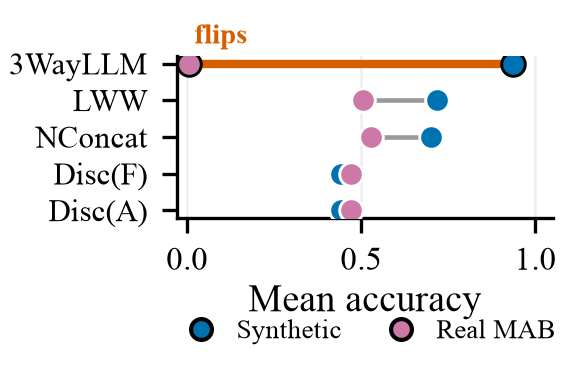
\includegraphics[width=\linewidth]{synthetic_vs_mab_a.png}
    \caption{All five strategies.}
    \label{fig:mab-negative-a}
  \end{subfigure}%
  \hfill
  \begin{subfigure}[b]{0.48\columnwidth}
    \centering
    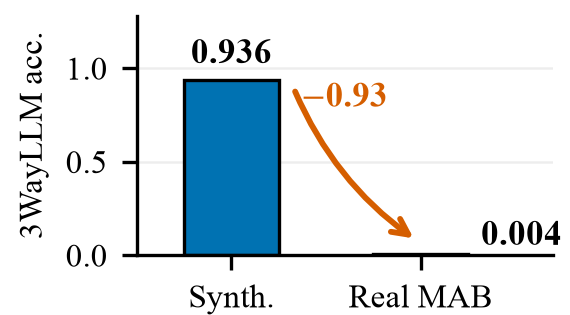
\includegraphics[width=\linewidth]{synthetic_vs_mab_b.png}
    \caption{\textsc{ThreeWayLLMMerge} alone.}
    \label{fig:mab-negative-b}
  \end{subfigure}
  \caption{Synthetic vs.\ real MemoryAgentBench. (a)
  \textsc{ThreeWayLLMMerge} goes from best to worst once the signal is
  removed. (b) Its accuracy drops $0.936\to0.004$ ($230$-conflict run;
  per-row spread in Appendix~\ref{sec:mab-per-row}).}
  \label{fig:mab-negative}
\end{figure}

\textsc{ThreeWayLLMMerge} scores a mean of $0.004$ accuracy on the expanded
sample ($1$ of $230$ correct) --- \emph{far below} every naive baseline (LWW
$0.506$, naive concat $0.528$, branch-discard $0.472$), the \emph{opposite}
ranking from the synthetic benchmark. Seven of eight real rows score
\emph{exactly} $0$, the eighth $0.033$ (Appendix~\ref{sec:mab-per-row}).
\textsc{ConfidenceRuleMerge} collapses identically, to exactly $0.000$,
confirming this is a property of the data, not an LLM-specific failure:
\texttt{mab\_extension.py} never constructs a source-reliability signal
(Section~\ref{sec:mab}), so every real conflict is an exact confidence tie,
which both strategies correctly refuse to break. It committed to a value
\emph{zero} times across all $230$ conflicts (Section~\ref{sec:abstention}
gives the full commit/abstention breakdown); naive baselines win only by
never abstaining --- we did not adjust the extension to flatter it; both
the $15$- and $50$-cap runs are released as-is.

\textbf{Reading:} RQ1's win is contingent on an explicit, legible reliability
signal we engineered into the synthetic benchmark. Absent it, the same
calibrated-caution behavior that scored $0.833$ on synthetic
\emph{ambiguous} conflicts becomes a liability under a scoring rule built
for \emph{resolvable} cases --- evidence real content may lack the assumed
signal, not poor reasoning. Appendix~\ref{sec:decision-matrix} gives a
condition-by-condition deployment recommendation.


\subsection{Abstention-aware evaluation}
\label{sec:abstention}

Raw accuracy scores a calibrated abstention identically to a confused guess:
both count as ``not correct.'' That conflation is exactly what makes
Section~\ref{sec:mab-negative}'s headline number ($0.004$) read as a
collapse in \emph{capability} rather than a shift in \emph{behavior}. We
report commit rate, conditional-on-commit accuracy, wrong-commit rate, and
expected utility under three wrong-commit costs ($-2$, $-5$, $-10$, against
$+1$ for a correct commit and $-1$ for abstaining) --- post-hoc, exploratory,
computed from already-cached model calls (Table~\ref{tab:abstention},
Figure~\ref{fig:abstention}; full metric definitions in
Appendix~\ref{sec:abstention-metrics-def}).

\begin{table}[H]
  \centering
  \small
  \resizebox{\columnwidth}{!}{%
  \begin{tabular}{lcc}
    \toprule
    \textbf{Metric} & \textbf{Synthetic ($n{=}180$)} & \textbf{Real MAB ($n{=}230$)} \\
    \midrule
    Commit rate            & $0.672$ & $0.000$ \\
    Cond.-on-commit acc.    & $0.835$ & undefined \\
    Wrong-commit rate       & $0.111$ & $0.000$ \\
    Flag precision          & $0.966$ & --- \\
    Flag recall             & $0.950$ & --- \\
    Expected utility ($-2$) & $+0.011$ & $-1.000$ \\
    Expected utility ($-5$) & $-0.322$ & $-1.000$ \\
    Expected utility ($-10$) & $-0.878$ & $-1.000$ \\
    \bottomrule
  \end{tabular}%
  }
  \caption{Abstention-aware metrics, \textsc{ThreeWayLLMMerge}. Synthetic
  pools resolvable+ambiguous ($n{=}60$ locked run; orthogonal excluded).
  Post-hoc, exploratory.}
  \label{tab:abstention}
\end{table}

\begin{figure}[H]
  \centering
  \begin{subfigure}[b]{0.48\columnwidth}
    \centering
    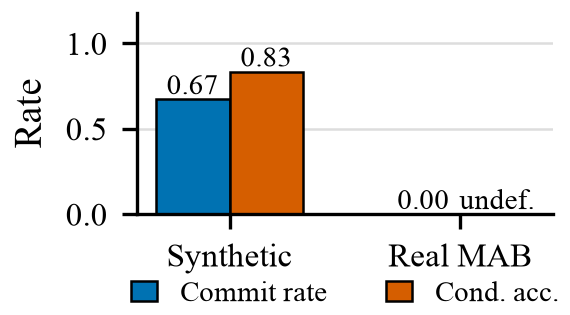
\includegraphics[width=\linewidth]{abstention_coverage.png}
    \caption{Commit rate vs.\ cond.\ accuracy.}
    \label{fig:abstention-a}
  \end{subfigure}%
  \hfill
  \begin{subfigure}[b]{0.48\columnwidth}
    \centering
    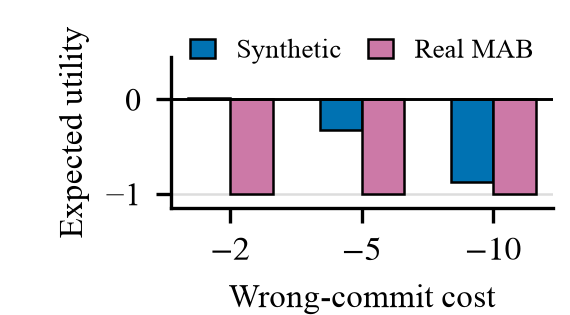
\includegraphics[width=\linewidth]{abstention_utility.png}
    \caption{Expected utility by cost.}
    \label{fig:abstention-b}
  \end{subfigure}
  \caption{(a) Conditional accuracy is high in both regimes ($0.835$
  synthetic; undefined on MAB, zero commits) --- not guessing worse, just
  committing less. (b) Full abstention (MAB) is a flat $-1$; synthetic
  utility falls \emph{below} that line once a wrong commit costs $10\times$
  an abstention.}
  \label{fig:abstention}
\end{figure}

The model's \emph{policy} is stable across settings: it commits and is
right most of the time when a signal exists (synthetic), and abstains
completely when it does not (MAB) --- consistent behavior, not degraded
reasoning. Whether that policy is \emph{good} depends on a cost structure
accuracy never asks about: at low wrong-commit cost, committing more beats
full abstention; at high cost, it does not. A deployment that cannot
specify its own wrong-commit cost cannot know which regime it is in ---
itself an argument for keeping \textsc{flagged\_unresolved} actionable
rather than silently resolved either way.

\section{Discussion}
\label{sec:discussion}

\paragraph{Construct validity is not free.} Building \textsc{BranchMem}
surfaced two piloting failures (and a third in Section~\ref{sec:semantic-resolvable-detail}).
First, a set-membership bug left every conflict targeting a brand-new key
with no ancestor value, so \textsc{ThreeWayLLMMerge} never received the
context it depends on --- invisible to unit tests with ancestor context
already wired in; only auditing transcripts, not aggregate scores, caught
it. Second, after the fix, three-way merge still scored near-zero on
resolvable conflicts, because ground truth had been a coin flip
indistinguishable from ``ambiguous.'' Tying it to an explicit
source-reliability signal ($15\%$ noise) is what makes RQ1 a real test.

\paragraph{Timestamps are a trap in the asynchronous case.} The
MAB-extension construction bugs (Section~\ref{sec:mab}) both accidentally
correlated a synthetic branch's timestamp with correctness, rigging LWW's
win or loss ($0.00$ or $1.00$); the fix randomized timestamp ordering
independent of correctness: recency is not evidence.

\paragraph{The MAB negative result is the same problem, and what the LLM
adds.} Section~\ref{sec:mab-negative}'s collapse to $0.004$ accuracy is the
same failure mode on real content: with no exposed reliability signal,
``resolvable'' is indistinguishable from ``ambiguous'' --- correctly to the
model, punitively to our scoring rule. We could fix this in piloting but
not on real content, so the synthetic design choice does more work than
Table~\ref{tab:confirmatory} suggests; we did not add a post-hoc rule
crediting calibrated abstention, since that is exactly the result-shopping
preregistration exists to prevent. The model's behavior is consistent
throughout: it reads resolvable conflicts well when the signal is present
and abstains when it is not --- only the scoring rule's reward changes, not
the model's judgment.

\section{Conclusion}
Three-way, ancestor-aware LLM merging wins decisively given a legible
reliability signal, and loses to every naive baseline once that signal is
gone. We take this as a boundary condition on RQ1, not a caveat to bury:
deployment needs either a genuine reliability signal in memory provenance,
or a downstream consumer that treats \textsc{flagged\_unresolved} as
actionable, not a failure.

\section*{Limitations}
\label{sec:limitations}

Our results come with real caveats, several preregistered, two added after
later post-hoc checks.

\noindent\textbf{Model coverage is still narrow.} The locked run uses one cheap
model (\texttt{gpt-5.4-nano}); the post-hoc \texttt{gpt-5.4-mini} check
(Section~\ref{sec:robustness}) reproduces RQ1's direction and magnitude, but is
a \emph{same-provider} swap only. No non-OpenAI API key is available in this
project's environment, so we could not and did not test any other model
family; every LLM-dependent number in this paper (RQ1, RQ3, the ablations,
and the RQ2 judge) is OpenAI-only, and whether the reported effects are
properties of LLMs reasoning about provenance in general, or specific to this
provider's small/cheap models, is untested and left to future work.

\noindent\textbf{The headline effect is contingent on an engineered signal,
demonstrated, not merely hypothesized.} Section~\ref{sec:mab-negative}'s
real-content analysis shows \textsc{ThreeWayLLMMerge} scoring \emph{below
every naive baseline} ($0.004$ vs.\ $0.47$--$0.53$) once the hand-designed
source-reliability signal is absent --- a measured boundary condition on RQ1,
the single most important caveat to this paper's aggregate numbers.

\noindent\textbf{Sample size and non-determinism.} The locked run is $n{=}60$
scenarios with each LLM call made once, not majority-voted; the pilot flip
rate was low ($6.7\%$), but reported numbers carry unquantified variance
beyond the paired bootstrap CI. The MAB secondary analysis
(Section~\ref{sec:mab-negative}) is smaller still ($8$ rows, capped at $50$
conflict keys per row for cost control via \texttt{max\_conflict\_keys}; an
initial $15$-cap pass, also released, agreed in direction and magnitude) and
used only \texttt{gpt-5.4-nano} (not the more capable \texttt{gpt-5.4-mini}
checked in Section~\ref{sec:robustness}); it is purely descriptive, with no
significance tests.

\noindent\textbf{No independent validation of ground truth.} All ground-truth
labels --- every ``resolvable'' case's correct answer, the $15\%$
source-signal noise parameter, and MemoryAgentBench's re-derived edit
chains --- are generated or parsed by construction in code, and no human
annotator is available in this project's environment to check any of them
independently. We did not substitute an LLM-based self-consistency check for
genuine human validation, since presenting one as the other would mislead.
What we did add: an \emph{author self-audit}
(not independent, not blind) of $50$ randomly sampled MemoryAgentBench
parser extractions against their source text, finding $0$ errors
($95\%$ Clopper--Pearson CI on the true error rate: $[0,0.071]$;
Section~\ref{sec:mab}). This bounds only whether the parser extracts what a
context line literally says, not whether ``resolvable'' ground truth or the
noise parameter reflect real-world provenance reliability, which remains
completely unvalidated. We provide an audit protocol and a sampled item set
(\texttt{annotation/audit\_sample.csv}, \texttt{annotation/audit\_instructions.md})
to support independent validation. We do not claim independent validation
was performed in this submission.

\noindent\textbf{H2's near-mechanical component.} As disclosed in advance, the
branch-discard effect is partly an artifact of the benchmark always including
orthogonal questions, not pure evidence about real-world information loss.

\noindent\textbf{NLI generalization gap.} The NLI detector's failure reflects
one fixed threshold from a modest calibration set, not necessarily an
intrinsic limit of NLI-based detection.

\noindent\textbf{Scoring-rule asymmetry.} Our scoring rule credits
\textsc{flagged\_unresolved} on the synthetic ambiguous category but treats it
as wrong on MemoryAgentBench's resolvable category --- an inconsistency in our
evaluation design, not just the two content sources; a consistent
abstention-crediting rule is future work.

\section*{Ethical Considerations}

\textsc{BranchMem} is a methods-and-benchmark paper. All scenarios in the locked
run are synthetically generated from a fixed template pool and contain no personal,
sensitive, or human-subject data; no human annotation was collected. The
MemoryAgentBench extension reuses a publicly released, MIT-licensed research
dataset within its intended research use. The only external service used is a
commercial LLM API, accessed under its terms; all calls are cached and committed
for auditability, and the run is inexpensive by design. We foresee no direct risk
of harm from this work; the broader technique---automatically merging an agent's
memory---should, in deployment, retain the human-in-the-loop \textsc{flag}
behavior our benchmark rewards, so that genuinely ambiguous conflicts are surfaced
rather than silently resolved.

\bibliography{custom}

\appendix

\section{ThreeWayLLMMerge Prompt}
\label{sec:prompt}

The system prompt instructs the model that it is reconciling two independently
updated branches of an agent's memory that diverged from a common ancestor while
disconnected. For each conflicting key it is given the ancestor value (or null),
and each branch's current value, \texttt{source}
(\texttt{user}/\texttt{observation}/\texttt{inference}), and \texttt{confidence}.
It is told to resolve using whatever signal actually distinguishes the two
updates---e.g.\ a user-sourced, higher-confidence update is ordinarily more
trustworthy than an inferred, lower-confidence one, and the ancestor value
indicates which branch's update is a genuine correction versus a stale
duplicate---and \emph{not} to use timestamps, since disconnected branches have no
shared clock. If source, confidence, and ancestor context give no real basis to
prefer one branch, it must flag the conflict unresolvable rather than guess. The
model returns strict JSON: for each key, one of
\{\texttt{kept\_from\_a}, \texttt{kept\_from\_b}, \texttt{merged},
\texttt{flagged\_unresolved}\}, a reconciled value (or null), and a one-sentence
justification. Non-conflicting keys are resolved in code and never sent to the
model. Below is the literal text, verbatim from \texttt{branchmem/merge/}
\texttt{three\_way\_llm.py} (constants \texttt{\_SYSTEM\_PROMPT} and
\texttt{\_PROMPT\_TEMPLATE}), so readers can judge instructions such as the
timestamp prohibition for themselves rather than trust our paraphrase.

\noindent\textbf{System prompt (verbatim).}\par
\nolinenumbers
\begin{lstlisting}
You are reconciling two independently-updated branches of an agent's memory that diverged from a common ancestor while disconnected from each other. For each conflicting (entity, predicate) key, you are given the common ancestor's value (if any) and each branch's current value, source, and confidence. 'source' is how that update was recorded: "user" means the user explicitly stated or corrected it; "inference" means the agent inferred or guessed it; "observation" means the agent observed it indirectly. Resolve each conflict using whatever signal actually distinguishes the two updates -- e.g. a user-sourced, higher-confidence update is ordinarily more trustworthy than an inferred, lower-confidence one; the ancestor value can indicate which branch's update is more likely a genuine correction vs. a stale duplicate. Do NOT use timestamps to decide, even if you can infer relative recency -- two branches that were disconnected from each other have no shared clock, so 'later' does not mean 'more correct' here. If source, confidence, and ancestor context give no real basis to prefer one branch over the other (e.g. both are equally plausible, equally-sourced preference changes), explicitly flag it as unresolvable rather than guessing.
\end{lstlisting}
\linenumbers


\noindent\textbf{User prompt template (verbatim, placeholders filled per merge call).}\par
\nolinenumbers

\begin{lstlisting}

Common ancestor value for each key (null if the key didn't exist yet):
{ancestor_json}

Branch A's current value/source/confidence for each conflicting key:
{branch_a_json}

Branch B's current value/source/confidence for each conflicting key:
{branch_b_json}

For EACH key listed above, decide how to reconcile it. Respond with strict JSON only,
no other text, in this exact shape:

{"resolutions": [
  {"entity": "...", "predicate": "...", "resolution": "kept_from_a" | "kept_from_b" | "merged" | "flagged_unresolved",
    "value": "<the reconciled value, or null if flagged_unresolved>", "justification": "<one sentence>"}
]}
\end{lstlisting}
\linenumbers
\texttt{\{ancestor\_json\}}, \texttt{\{branch\_a\_json\}}, and
\texttt{\{branch\_b\_json\}} are substituted at call time with the actual
per-key JSON blocks for that merge's conflicting keys only; non-conflicting
keys are never sent to the model. Appendix~\ref{sec:example} shows one such
call filled in, with the model's real response.

\section{Worked Example}
\label{sec:example}

To make the mechanism concrete rather than only described in the abstract, this
is one real, representative transcript from the committed model-call cache
(\texttt{llm\_cache/}, content-hash addressed and described in Section~\ref{sec:results}'s
Reproducibility paragraph), reproduced verbatim. The individual cache entry does
not retain a back-link to a specific locked-run \texttt{scenario\_id}, so we
present it as illustrative of the mechanism rather than tied to one row of
Table~\ref{tab:category}; its pattern (source/confidence resolves two keys,
symmetric equal-source conflict gets flagged) matches the aggregate category
behavior reported there.

\paragraph{Inputs sent to the model.} One entity (\texttt{erin}) with three
conflicting keys. The ancestor only had a value for one of them
(\texttt{opinion\_of\_new\_policy = "neutral"}); the other two are new keys
each branch introduced independently, so the ancestor value is absent for
those.

\begin{center}
\small
\begin{tabular}{@{}lllc@{}}
\toprule
\textbf{Key} & \textbf{Branch A} & \textbf{Branch B} & \textbf{Ancestor} \\
\midrule
manager\_name & \emph{riley chen} & \emph{taylor reyes} & --- \\
 & \scriptsize user, $0.95$ & \scriptsize inference, $0.55$ & \\
opinion\_of\_ & \emph{skeptical} & \emph{supportive} & \emph{neutral} \\
new\_policy & \scriptsize observation, $0.7$ & \scriptsize observation, $0.7$ & \\
phone\_number & \emph{555-0142} & \emph{555-0101} & --- \\
 & \scriptsize inference, $0.55$ & \scriptsize user, $0.95$ & \\
\bottomrule
\end{tabular}
\end{center}

\paragraph{Model's actual response (verbatim \texttt{justification} fields).}
\begin{itemize}[itemsep=2pt,topsep=2pt]
  \item \textbf{manager\_name} $\to$ \textsc{kept\_from\_a}, ``riley chen'':
  \emph{``Branch A is user-sourced with higher confidence (0.95) than Branch
  B's inference (0.55).''}
  \item \textbf{opinion\_of\_new\_policy} $\to$ \textsc{flagged\_unresolved}:
  \emph{``Both branches are observation-sourced with equal confidence (0.7)
  and the ancestor value ('neutral') does not distinguish which is
  correct.''}
  \item \textbf{phone\_number} $\to$ \textsc{kept\_from\_b}, ``555-0101'':
  \emph{``Branch B is user-sourced with higher confidence (0.95) than Branch
  A's inference (0.55).''}
\end{itemize}
All three justifications cite exactly the signal the system prompt says to
use (source and confidence) and nothing else; none mentions recency, even
though the model is not shown timestamps at all for these keys. The two
resolvable conflicts are resolved toward whichever branch is user-sourced and
higher-confidence, regardless of whether that is Branch A or Branch B --- the
model is not simply defaulting to one branch. The third key is a textbook
ambiguous case in our taxonomy (Section~\ref{sec:gen}): identical source,
identical confidence, uninformative ancestor --- and the model flags it
instead of guessing, exactly the behavior Section~\ref{sec:mab-negative}
shows becoming costly once the scoring rule assumes a signal is present.

\section{Per-Divergence-Span Results}
\label{sec:per-span}

Section~\ref{sec:results} reports that divergence duration had little effect
on \textsc{ThreeWayLLMMerge} ($0.914/0.957/0.936$ at spans $4.0/10.0/20.0$).
Table~\ref{tab:per-span} gives the same breakdown for all five strategies,
computed from the locked run's per-scenario records in
\texttt{results/final/results.json} ($20$ scenarios per span, $60$ total).
No strategy's ranking changes across spans, and \textsc{ThreeWayLLMMerge}'s
own accuracy varies by only $0.043$ across a $5\times$ range of divergence
duration --- consistent with the aggregate result not being an artifact of a
particular span.

\begin{table}[t]
\centering
\small
\resizebox{\columnwidth}{!}{%
\begin{tabular}{lccc}
\toprule
\textbf{Strategy} & \textbf{span 4.0} & \textbf{span 10.0} & \textbf{span 20.0} \\
\midrule
last\_writer\_wins            & $0.700$ & $0.736$ & $0.714$ \\
naive\_concat                 & $0.707$ & $0.700$ & $0.693$ \\
branch\_discard (always\_b)   & $0.436$ & $0.443$ & $0.450$ \\
branch\_discard (fewer\_upd.) & $0.436$ & $0.443$ & $0.450$ \\
three\_way\_llm               & $0.914$ & $0.957$ & $0.936$ \\
\bottomrule
\end{tabular}%
}
\caption{Accuracy by divergence span and strategy ($20$ scenarios/span).
Descriptive; span was not a preregistered factor.}
\label{tab:per-span}
\end{table}

\section{MemoryAgentBench Per-Row Detail}
\label{sec:mab-per-row}

Section~\ref{sec:mab-negative}'s headline number ($0.004$ mean accuracy for
\textsc{ThreeWayLLMMerge}) is a mean over only $8$ real Conflict\_Resolution
rows --- the full dataset, not a subsample. Table~\ref{tab:mab-per-row} gives
the individual rows from the expanded run
(\texttt{mab\_secondary\_analysis\_expanded.json}, \texttt{max\_conflict\_keys}${=}50$,
$230$ total conflicts), to make the spread behind that mean transparent
rather than reporting only the aggregate.

\begin{table}[t]
\centering
\small
\begin{tabular}{cccc}
\toprule
\textbf{Row} & \textbf{$n$ pairs} & \textbf{$n$ questions} & \textbf{3-way acc.} \\
\midrule
0 & $29$ & $29$ & $0.000$ \\
1 & $23$ & $23$ & $0.000$ \\
2 & $27$ & $27$ & $0.000$ \\
3 & $30$ & $30$ & $0.033$ \\
4 & $29$ & $29$ & $0.000$ \\
5 & $26$ & $26$ & $0.000$ \\
6 & $35$ & $35$ & $0.000$ \\
7 & $31$ & $31$ & $0.000$ \\
\bottomrule
\end{tabular}
\caption{Per-row detail behind Section~\ref{sec:mab-negative}'s $0.004$ mean
(\texttt{max\_conflict\_keys}${=}50$). Other strategies
(\textsc{ConfidenceRuleMerge} scores $0.000$ throughout) are in the released
JSON. An earlier pass ($15$-cap, $67$ conflicts, mean $0.056$) agrees in
direction and magnitude.}
\label{tab:mab-per-row}
\end{table}

\noindent Seven of eight rows score exactly $0$; row $3$ is the only
exception, at $0.033$ ($1$ of $30$ questions). This is not one degenerate row
dragging down an otherwise-healthy mean --- the near-uniform floor is what we
would expect if the mechanism identified in Section~\ref{sec:mab-negative} (no
source-reliability signal to read, so the model flags almost every conflict)
operates consistently across rows. Splitting by commit/flag makes this
precise: across all $230$ conflicts, \textsc{ThreeWayLLMMerge} \emph{committed
to an answer zero times} --- every single response was
\textsc{flagged\_unresolved}. Its conditional-on-commit accuracy is therefore
undefined, not merely low; there were no commits to be accurate or inaccurate
about. This is stronger and more mechanically legible evidence than the
$n{=}8$-row aggregate alone would suggest, since it does not depend on
between-row averaging at all. We did not measure per-row parser coverage
separately; only the aggregate figure reported in Section~\ref{sec:mab}
($99.9\%$ over $18{,}337$ unique context
lines, across the full dataset the $8$ rows are drawn from) was logged.

\section{Detector Threshold Calibration Sweep}
\label{sec:calibration}

Section~\ref{sec:results} states embedding and NLI thresholds were chosen
from a plateau rather than an edge value. Table~\ref{tab:calibration} gives
the sweep behind that claim, against the $60$ ground-truth conflict pairs in
the held-out pilot set (\texttt{ANALYSIS\_PLAN.md} \S3). Precision was
$1.0$ at every threshold tested for both detectors --- across the entire
sweep, neither detector ever produced a false positive; all sweep error is
missed conflicts (false negatives).

\textbf{Judge F1 drift, bootstrapped.} On the pilot calibration set, both
cheap detectors tied at F1 $0.938$ against an uncalibrated-default judge F1
of $0.966$ (gaps $\approx0.028$, both inside the $0.05$ tolerance); on the
independently-generated, three-times-larger locked set, the judge's own F1
rose to $0.986$. Bootstrapped $95\%$
CIs ($2000$ resamples) show why this need not be systematic: judge F1
$0.966$ $[0.929,0.992]$ (pilot) vs.\ $0.986$ $[0.971,0.997]$ (locked)
overlap substantially, consistent with ordinary sampling variation at
$3\times$ the sample size. The gap itself bootstraps to $0.029$
$[0.006,0.056]$ (embedding) and $0.061$ $[0.036,0.089]$ (NLI).

\begin{table}[t]
\centering
\small
\begin{tabular}{lcc}
\toprule
\textbf{Threshold band} & \textbf{Embedding F1} & \textbf{NLI F1} \\
\midrule
$0.10$--$0.25$ & --- & $0.938$ \\
$0.30$--$0.55$ & --- & $0.929$ \\
$0.60$--$0.75$ & --- & $0.919$ \\
$0.80$--$0.90$ & $0.938$ & $0.909$ \\
\bottomrule
\end{tabular}
\caption{Pilot-set F1 by threshold band (embedding swept $[0.30,0.90]$, NLI
$[0.10,0.90]$, step $0.05$). Embedding flat at $0.938$ from $0.80$ up; NLI
peaked at $0.938$ for $0.10$--$0.25$, declining above. Locked: embedding
$0.80$, NLI $0.20$ --- plateau interiors chosen for robustness, not the
single best pilot value.}
\label{tab:calibration}
\end{table}

\section{Locked Scenario Configuration}
\label{sec:config}

The locked run used: $1$ entity, $4$ ancestor facts, $2$ orthogonal additions per
branch, $2$ resolvable conflicts, $1$ ambiguous conflict, timestamp--correctness
correlation ${=}0.5$, source-signal noise ${=}0.15$, over three divergence spans
$\{4.0, 10.0, 20.0\}$ ($20$ scenarios each, $n{=}60$ total, $180$ conflict pairs:
$120$ resolvable, $60$ ambiguous), seed $2026$. Detector thresholds: embedding
$0.80$, NLI $0.20$, calibrated on the held-out pilot set.

\textbf{Documentation correction (found during this revision).}
\texttt{ANALYSIS\_PLAN.md} \S1 documented one orthogonal addition per branch;
re-auditing \texttt{scripts/run\_experiment.py} found it never overrides
\texttt{ScenarioConfig}'s orthogonal-count defaults, so two per branch
actually ran (confirmed empirically: \texttt{results/final/results.json}'s
per-scenario question count is $7{=}2{+}2{+}2{+}1$, not $5{=}1{+}1{+}2{+}1$).
This is a documentation error, not a results change --- every accuracy number
in this paper is computed correctly from what actually ran; only the earlier
prose description of the config (here and in \texttt{ANALYSIS\_PLAN.md}) was
wrong. It does not affect any conclusion: the orthogonal category is tied at
$1.000$ across every strategy regardless of whether $2$ or $4$ orthogonal
keys are involved.

\section{Deployment Decision Matrix}
\label{sec:decision-matrix}

Table~\ref{tab:decision-matrix} translates Section~\ref{sec:mab-negative}'s
boundary condition into condition-by-condition guidance for a system builder
deciding how to consume \textsc{ThreeWayLLMMerge}'s output.

\begin{table}[t]
  \centering
  \small
  \begin{tabular}{p{0.44\columnwidth}p{0.42\columnwidth}}
    \toprule
    \textbf{Condition} & \textbf{Recommended behavior} \\
    \midrule
    Reliable provenance available (distinguishable source/confidence) &
      Three-way merge can resolve; expect accuracy near the synthetic
      resolvable-conflict result ($0.858$). \\
    \addlinespace
    No provenance, or equal confidence on both branches &
      Do not force a resolution; flag. Committing anyway is indistinguishable
      from guessing (Section~\ref{sec:mab-negative}). \\
    \addlinespace
    Downstream consumer can act on an unresolved flag &
      Treat the flag as a successful outcome, not a failure --- it is the
      correct output when no signal exists. \\
    \addlinespace
    Downstream consumer requires a forced single answer &
      A naive baseline (LWW, concat) may score higher under accuracy-only
      metrics, but this reflects the metric, not increased safety --- see
      Section~\ref{sec:discussion}'s scoring-rule asymmetry. \\
    \bottomrule
  \end{tabular}
  \caption{Deployment guidance implied by RQ1's boundary condition.}
  \label{tab:decision-matrix}
\end{table}

\section{Resolvable-Category Power Expansion Detail}
\label{sec:power-expansion-detail}

Full per-strategy numbers for the post-hoc power-expansion replication
(Section~\ref{sec:power-expansion}): base seed $2029$, $120$ new resolvable
pairs, kept disjoint from and not pooled with the locked ($n{=}60$, seed
$2026$) run. Dashes mark strategies for which the locked run's per-scenario
logs recorded only overall (not per-category) accuracy, so a resolvable-only
locked-run figure is not available for direct comparison; the new sample's
own significance tests (below the table) are self-contained and do not rely
on that comparison.

\begin{table}[t]
  \centering
  \small
  \resizebox{\columnwidth}{!}{%
  \begin{tabular}{lcc}
    \toprule
    \textbf{Strategy} & \textbf{New sample} & \textbf{Locked run} \\
    \midrule
    \textsc{ThreeWayLLMMerge}      & $0.908$ & $0.858$ \\
    \textsc{ConfidenceRuleMerge}   & $0.917$ & --- \\
    \textsc{TwoWayLLMMerge}        & $0.917$ & --- \\
    \textsc{RawTextLLMMerge}       & $0.000$ & --- \\
    last\_writer\_wins             & $0.483$ & $0.508$ \\
    naive\_concat                  & $0.417$ & $0.450$ \\
    branch\_discard (both)         & $0.583$ & $0.550$ \\
    \bottomrule
  \end{tabular}%
  }
  \caption{Resolvable-only accuracy, new $n{=}120$ sample vs.\ locked
  $n{=}120$. On the new sample, \textsc{ConfidenceRuleMerge} and
  \textsc{TwoWayLLMMerge} both tie \textsc{ThreeWayLLMMerge}
  ($p{=}0.317$ both, diff $-0.008$); \textsc{RawTextLLMMerge} again scores
  $0.000$. All four naive-baseline differences vs.\ \textsc{ThreeWayLLMMerge}
  are large and significant (Wilcoxon $p<10^{-5}$; e.g.\ vs.\
  last\_writer\_wins: diff $+0.425$, $95\%$ CI $[0.325,0.525]$).}
  \label{tab:power-expansion}
\end{table}

\section{Balanced Detector Benchmark Detail}
\label{sec:detectors-balanced-detail}

Section~\ref{sec:detectors-balanced}'s locked set has no negative examples
by construction, so precision is mechanically $1.0$ for every detector ---
it measures recall only. We built a balanced, hand-authored $48$-pair set
across six categories: genuine contradiction and subtle ambiguous conflict
as true positives ($n{=}16$), and paraphrase, entailment,
unrelated-same-entity content, and preference refinement as true negatives
($n{=}32$), then re-ran all three detectors (post-hoc, exploratory; does
not change or retract RQ2's locked result). Full metrics below.

\begin{table}[H]
  \centering
  \small
  \resizebox{\columnwidth}{!}{%
  \begin{tabular}{lccccc}
    \toprule
    \textbf{Detector} & \textbf{Prec.} & \textbf{Rec.} & \textbf{F1} & \textbf{Spec.} & \textbf{AUROC} \\
    \midrule
    embedding ($t{=}0.80$) & $0.381$ & $1.000$ & $0.552$ & $0.188$ & $0.463$ \\
    NLI ($t{=}0.20$)       & $0.667$ & $1.000$ & $0.800$ & $0.750$ & $0.871$ \\
    LLM judge              & $0.722$ & $0.813$ & $0.765$ & $0.844$ & $0.828^\dagger$ \\
    \bottomrule
  \end{tabular}%
  }
  \caption{Balanced detector benchmark ($48$ pairs, $16$ conflict / $32$
  non-conflict). $^\dagger$LLM judge emits a binary score only, so its
  AUROC collapses to a single operating point rather than a true ranked
  curve; reported for completeness, not read as equivalent to the
  continuous-score detectors' AUROC.}
  \label{tab:detectors-balanced}
\end{table}

Per-category accuracy: embedding scores $1.0$ on contradiction and
ambiguous-conflict but only $0.125$ on paraphrase and entailment, $0.5$ on
preference-refinement, and $0.0$ on unrelated-same-entity (it measures
surface dissimilarity, not semantic incompatibility, so it flags most
non-conflicts as conflicts). NLI scores $1.0$ on every category except
unrelated-same-entity ($0.0$). The LLM judge scores $0.875$ on
contradiction, $1.0$ on paraphrase and preference-refinement, $0.875$ on
entailment, $0.75$ on ambiguous-conflict, and $0.5$ on unrelated-same-entity
--- the most even profile of the three, but no detector handles unrelated
content sharing an entity and predicate well, since none of the three
signals was built to distinguish ``irrelevant'' from ``incompatible.''

\section{Semantic-Resolvable Category Detail}
\label{sec:semantic-resolvable-detail}

Full construction and transcript detail for Section~\ref{sec:semantic-resolvable}'s
\texttt{semantic\_resolvable} category ($n{=}150$, seed $3001$, disjoint
from the locked run's $2026$): both branches get identical source
(\texttt{observation}) and confidence ($0.7$), and independently-randomized
timestamps, so no structured field distinguishes them.

\textbf{A construct-validity bug we caught and fixed.} The first version of
this experiment stored the ancestor's constraint under a \emph{different}
predicate than the conflicting key (e.g.\ \texttt{dietary\_preference} vs.\
\texttt{dinner\_choice}). \textsc{ThreeWayLLMMerge}'s prompt includes the
ancestor's value only for the exact colliding key
(Section~\ref{sec:formulation}), so the constraint was invisible to the
model regardless of its reasoning ability --- a bug in our harness, not a
finding about semantic reasoning, in the same family as
Section~\ref{sec:discussion}'s piloting bugs. We caught it by inspecting a
cached response directly rather than trusting the aggregate $0.000$,
rewrote the templates so the constraint lives at the conflicting key, and
re-ran (new API calls; both the flawed and corrected runs are cached under
\texttt{llm\_cache/} and released).

\textbf{Result after the fix.} Every confidence-independent strategy still
scores \emph{exactly} $0.000$: \textsc{ConfidenceRuleMerge} correctly flags
the equal-confidence tie (as designed); \textsc{TwoWayLLMMerge} and
\textsc{RawTextLLMMerge} structurally lack the ancestor content needed
here; and --- the more informative result ---
\textsc{ThreeWayLLMMerge}, which \emph{does} receive the constraint, also
scores $0$. Inspecting individual transcripts shows inconsistent, not
absent, behavior: some conflicts are correctly flagged; some are merged
into an incoherent combination of both values (e.g.\ ``wants chicken for
dinner and wants tofu for dinner''); and at least one is a confident
\emph{wrong} commit that ignores a stated allergy constraint entirely. This
sharpens rather than undercuts RQ1's reframing
(Section~\ref{sec:ablations}): the LLM's aggregate advantage over naive
baselines is attributable to reading a structured confidence field, and we
found no category in this benchmark, semantic or otherwise, where its
raw-text reasoning reliably exceeds that.

\section{Abstention Metric Definitions}
\label{sec:abstention-metrics-def}

Metrics reported in Section~\ref{sec:abstention} (Table~\ref{tab:abstention}),
computed by \texttt{branchmem/eval/abstention\_metrics.py} over pooled
resolvable+ambiguous downstream questions (orthogonal excluded --- there is
nothing to abstain from). Let $N$ be the number of in-scope questions,
$C$ the number committed (resolution $\neq$ \textsc{flagged\_unresolved}),
$C_{\text{correct}}$ the number of those that are correct, and
$F = N - C$ the number flagged.

\begin{itemize}[itemsep=1pt,topsep=2pt,leftmargin=*]
  \item \textbf{Commit rate} $= C / N$. \textbf{Abstention rate} $= F / N$.
  \item \textbf{Conditional-on-commit accuracy} $= C_{\text{correct}} / C$
  (undefined, not zero, when $C{=}0$).
  \item \textbf{Wrong-commit rate} $= (C - C_{\text{correct}}) / N$.
  \item \textbf{Flag precision} $=$ (flags on genuinely ambiguous questions)
  $/ F$. \textbf{Flag recall} $=$ (ambiguous questions flagged) $/$ (total
  ambiguous questions) --- equivalent to the ambiguous-category accuracy in
  Table~\ref{tab:category}.
  \item \textbf{Expected utility} (per question, averaged over $N$): a
  correct commit scores $+1$, an abstention scores $-1$, and a wrong commit
  scores the regime's cost ($-2$, $-5$, or $-10$ in Table~\ref{tab:abstention}).
  \item \textbf{Coverage} $=$ commit rate. \textbf{Risk} $= 1 -$
  conditional-on-commit accuracy (undefined when coverage is $0$), following
  the risk-coverage framing of selective classification
  \citep{elyaniv2010selective,geifman2017selective}.
\end{itemize}

All metrics here are post-hoc and exploratory (ANALYSIS\_PLAN\_ADDENDUM.md,
item A1); none are part of ANALYSIS\_PLAN.md's confirmatory tests.

\section{Extended Related Work}
\label{sec:related-work-extended}

Full discussion of four related-work points introduced briefly in
Section~\ref{sec:related-work}, moved here since each is either already
distinguished from our setting in Section~\ref{sec:intro}, or is
background supporting a single RQ rather than the paper's central boundary-
condition claim.

\subsection{Agent memory and memory benchmarks}
Reflexion \citep{shinn2023reflexion} and MemGPT \citep{packer2023memgpt}
give single agents persistent, self-managed memory --- verbal
self-reflection and OS-inspired paging --- but assume one continuously-
running agent, not two independently-updated copies to reconcile.
MemoryAgentBench \citep{hu2025memoryagentbench} benchmarks retrieval,
test-time learning, long-range understanding, and selective forgetting for
such single-timeline agents; its Fact Consolidation task is our extension's
raw material (Section~\ref{sec:mab}).

\subsection{Live multi-agent coordination vs.\ offline branch reconciliation}
S-Bus \citep{khan2026sbus} targets concurrent LLM agents sharing mutable
state over a common substrate: it reconstructs each agent's read set and
uses optimistic concurrency control to abort or retry conflicting commits
--- a \emph{prevention/abort} model for agents online together. Our
branches already committed divergent histories offline, so abort is not an
option; \textsc{BranchDiscard} is the natural post-hoc analogue, testing
whether that cheap move is good enough (RQ3).

\subsection{Single-timeline freshness and temporal conflict resolution}
\citet{reddy2026freshness} show that for a single-timeline list where a
counterfactual edit gets a higher serial, a deterministic ``pick the
maximum serial'' rule beats LLM judgement. Our problem lacks such an order:
asynchronous branches carry independent local clocks, so recency is
uninformative by construction (Section~\ref{sec:gen}).

\subsection{Conflict detection, NLI, and semantic similarity}
Prior work studies conflicts between an LLM's parametric knowledge and
retrieved context \citep{longpre2021knowledge}, and retrieval-augmented
generation \citep{lewis2020rag} --- model memory vs.\ an external source at
inference time. We instead study conflict between two versions of an
agent's \emph{own} memory that diverged offline. Our cheap detectors (RQ2)
build on sentence embeddings \citep{reimers2019sentencebert} and NLI-style
contradiction scoring; Section~\ref{sec:detectors-balanced}'s balanced
benchmark tests both against non-conflict categories this line of work is
designed to not flag.

\section{Post-hoc Robustness Checks Detail}
\label{sec:robustness-detail}

Full setup and figures for Section~\ref{sec:robustness}'s two post-hoc
robustness checks.

\subsection{A more capable model}
We ran \texttt{gpt-5.4-mini} in place of \texttt{gpt-5.4-nano} for
\textsc{ThreeWayLLMMerge} on the same $20$ scenarios (divergence span
$4.0$), everything else identical. Figure~\ref{fig:robustness} shows the
result is reassuring but modest: mean accuracy $0.929$ (mini) vs.\ $0.914$
(nano), paired difference $+0.014$, $95\%$ CI $[-0.014, 0.043]$, Wilcoxon
$p=0.45$ --- not distinguishable from noise. The direction and magnitude of
RQ1 hold with a more capable model, and a \emph{same-provider} check only
--- we did not have access to a different model family for this study.

\begin{figure}[H]
  \centering
  \begin{subfigure}[b]{0.48\columnwidth}
    \centering
    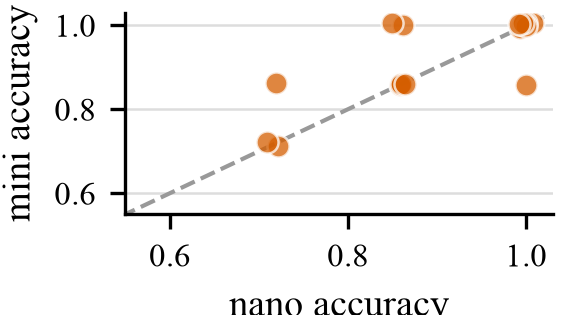
\includegraphics[width=\linewidth]{robustness_a.png}
    \caption{Per-scenario accuracy.}
    \label{fig:robustness-a}
  \end{subfigure}%
  \hfill
  \begin{subfigure}[b]{0.48\columnwidth}
    \centering
    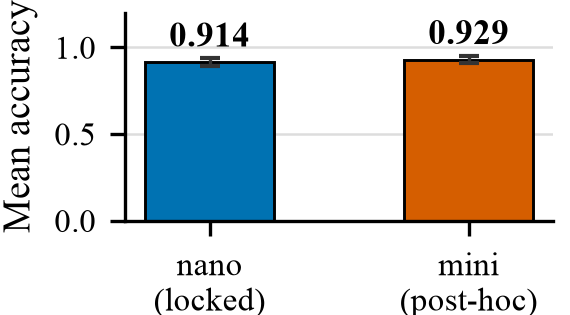
\includegraphics[width=\linewidth]{robustness_b.png}
    \caption{Mean accuracy.}
    \label{fig:robustness-b}
  \end{subfigure}
  \caption{\texttt{gpt-5.4-mini} vs.\ locked \texttt{gpt-5.4-nano}, same
  $20$ scenarios. Paired diff.\ $+0.014$, $95\%$ CI $[-0.014,0.043]$,
  $p=0.45$: small, not significant.}
  \label{fig:robustness}
\end{figure}

\subsection{A resolvable-category replication}
Since the resolvable category carries essentially all of RQ1's
non-mechanical evidence, we generated a second, disjoint-seed sample
($120$ new resolvable pairs, base seed $2029$) for more statistical power.
Post-hoc, kept separate from Tables~\ref{tab:confirmatory}--\ref{tab:category}:
it replicates closely ($0.908$ resolvable-only vs.\ $0.858$ locked, all four
naive-baseline differences remain large and significant alone, Wilcoxon
$p{<}10^{-5}$; \textsc{ConfidenceRuleMerge}/\textsc{TwoWayLLMMerge} again
land within noise of it, $p{=}0.32$ both; \textsc{RawTextLLMMerge} again
scores exactly $0.000$) --- $240$ independently-drawn resolvable pairs
total, every qualitative conclusion unchanged. Full numbers in
Table~\ref{tab:power-expansion}, Appendix~\ref{sec:power-expansion-detail}.

\end{document}
